\documentclass[11pt]{article}
\usepackage[letterpaper,margin=2cm]{geometry}
\usepackage[english]{babel}
\usepackage[utf8]{inputenc}
\usepackage[T1]{fontenc}
\linespread{1.3}
\parskip=12pt
\parindent=0pt
\usepackage{enumerate}
\usepackage{amsmath}
\usepackage{amsfonts}
\usepackage{graphicx}
\usepackage[section]{placeins}
\usepackage{amsthm}
\usepackage{amssymb}
\usepackage{mathpazo}
\usepackage{booktabs}
\usepackage{float}
\usepackage{listings}

\usepackage[dvipsnames]{xcolor}
\definecolor{slateblue}{RGB}{45, 62, 80}
\definecolor{FGVBlue}{RGB}{0, 114, 188}
\usepackage{hyperref}
\hypersetup{
	colorlinks=true,
	linkcolor=FGVBlue,
	urlcolor=FGVBlue,
	citecolor=FGVBlue,
}

\lstset{language=R, basicstyle=\ttfamily\footnotesize, breaklines=true,
	commentstyle=\color{gray}, keywordstyle=\color{slateblue}\bfseries,
	frame=single, rulecolor=\color{lightgray}, columns=fullflexible, keepspaces=true,
	showstringspaces=false}

% Custom commands
\newcommand{\E}{\mathbb{E}}
\newcommand{\Var}{\mathrm{Var}}
\newcommand{\Cov}{\mathrm{Cov}}
\newcommand{\Prob}{\mathbb{P}}
\newcommand{\symbf}[1]{\boldsymbol{#1}}

\newcounter{problem}
\renewcommand{\theproblem}{\arabic{problem}}
\newcommand{\problem}{
	\stepcounter{problem}
	\section*{Problem \theproblem}
}
\newcommand{\itm}[1]{\par\textbf{#1)}\ }
% Expandable \input, so that table rows can be read inside a tabular
\makeatletter
\newcommand{\tablerows}[1]{\@@input #1 }
\makeatother

\begin{document}
	\begin{center}
		{\LARGE{\textbf{Problem Set III -- Solutions}}}\\
		\vspace{0.2cm}
		Econometrics I - \textcolor{FGVBlue}{FGV EPGE}\\
		Instructor: Raul Guarini Riva \\
		TA: Taric Latif Padovani
	\end{center}

The code for Problems 3, 4 and 5 is in R and is reproduced at the end of each problem. Simulations use \texttt{set.seed(2026)}, so the numbers below are exactly reproducible. The IPCA data run from February 1995 to September 2026 ($T=380$ months).

%=====================================================================
\problem

\itm{a}
Let $A$ be the \emph{companion matrix} and $U_t$ the shock vector:
\[
A=\begin{pmatrix}
\phi_1&\phi_2&\cdots&\phi_{p-1}&\phi_p\\
1&0&\cdots&0&0\\
0&1&\cdots&0&0\\
\vdots&&\ddots&&\vdots\\
0&0&\cdots&1&0
\end{pmatrix},\qquad
U_t=\begin{pmatrix}\varepsilon_t\\0\\\vdots\\0\end{pmatrix}.
\]
The first row of $Y_t=AY_{t-1}+U_t$ is the AR($p$) equation, $y_t-\mu=\sum_i\phi_i(y_{t-i}-\mu)+\varepsilon_t$. Row $k\ge2$ reads $y_{t-k+1}-\mu=y_{t-k+1}-\mu$: it just shifts each lag down one position. Since only the first entry of $U_t$ is nonzero, $U_tU_t'$ has $\varepsilon_t^2$ in position $(1,1)$ and zeros elsewhere, so $\Omega=\E[U_tU_t']=\mathrm{diag}(\sigma^2,0,\dots,0)$.

\itm{b}
Iterating $h$ times,
\[
Y_{t+h}=A^hY_t+\sum_{j=0}^{h-1}A^jU_{t+h-j}.
\]
$Y_t$ is known at time $t$. The future shocks $\varepsilon_{t+1},\dots,\varepsilon_{t+h}$ are independent of $\mathcal I_t$ (the $y$'s up to $t$ depend only on shocks dated $t$ or earlier) and have mean zero. Hence $\E[Y_{t+h}\mid\mathcal I_t]=A^hY_t$.

\itm{c}
Given $\mathcal I_t$, only the sum of future shocks is random. The $U_{t+h-j}$'s are independent across $j$, so the cross terms vanish and
\[
\Var[Y_{t+h}\mid\mathcal I_t]=\sum_{j=0}^{h-1}A^j\,\Omega\,(A^j)' .
\]
Its $(1,1)$ element is the variance of the $h$-step forecast error of $y$. Since $(A^j)_{11}=\psi_j$, the $j$-th MA($\infty$) coefficient, it equals $\sigma^2\sum_{j=0}^{h-1}\psi_j^2$.

\itm{d}
Write
\[
A-\lambda I=\begin{pmatrix}
\phi_1-\lambda&\phi_2&\cdots&\phi_{p-1}&\phi_p\\
1&-\lambda&\cdots&0&0\\
\vdots&\ddots&\ddots&&\vdots\\
0&\cdots&1&-\lambda&0\\
0&\cdots&0&1&-\lambda
\end{pmatrix}.
\]
Take $\lambda\neq0$. Add $\frac1\lambda\times$(column $p$) to column $p-1$: this zeros the $1$ in row $p$, and the first-row entry becomes $\phi_{p-1}+\phi_p/\lambda$. Then add $\frac1\lambda\times$(the new column $p-1$) to column $p-2$, which zeros the $1$ in row $p-1$, and so on, down to column 1. These operations do not change the determinant, and they leave an upper triangular matrix with diagonal
\[
\Big(\phi_1-\lambda+\frac{\phi_2}{\lambda}+\frac{\phi_3}{\lambda^2}+\cdots+\frac{\phi_p}{\lambda^{p-1}},\ -\lambda,\ \dots,\ -\lambda\Big).
\]
Hence
\[
\det(A-\lambda I)=(-\lambda)^{p-1}\Big(\phi_1-\lambda+\sum_{j=2}^p\phi_j\lambda^{1-j}\Big)
=(-1)^{p}\big(\lambda^p-\phi_1\lambda^{p-1}-\phi_2\lambda^{p-2}-\cdots-\phi_p\big)=\Phi(\lambda).
\]
Both sides are polynomials in $\lambda$ that agree for every $\lambda\neq0$, so they agree at $\lambda=0$ too. The eigenvalues of $A$ are the roots of $\Phi$.

\itm{e}
Stationarity of the AR($p$) means that the roots of $f(z)=1-\phi_1z-\cdots-\phi_pz^p$ lie outside the unit circle. By d), the eigenvalues of $A$ are the roots of $z^p-\phi_1z^{p-1}-\cdots-\phi_p=z^pf(1/z)$, the polynomial with the coefficients of $f$ in reverse order. By Problem 4 of Problem Set II, its roots are the inverses of the roots of $f$, so they all lie inside the unit circle.

\itm{f}
All eigenvalues of $A$ have modulus below one, so $A^h\to0$. (If $A=P\Lambda P^{-1}$ is diagonalizable, $A^h=P\Lambda^hP^{-1}$; in general, the Jordan form gives entries of the form $h^k\lambda^h$, which still go to zero.) Hence
\[
\E[Y_{t+h}\mid\mathcal I_t]=A^hY_t\to0,\qquad\text{that is,}\qquad\E[y_{t+h}\mid\mathcal I_t]\to\mu,
\]
\[
\Var[Y_{t+h}\mid\mathcal I_t]\to\Gamma\equiv\sum_{j=0}^\infty A^j\,\Omega\,(A^j)' ,
\]
which converges because $\|A^j\|$ decays geometrically. $\Gamma$ is the unconditional variance of $Y_t$: it solves $\Gamma=A\Gamma A'+\Omega$, which is $\Var(Y_t)=\Var(AY_{t-1}+U_t)$ for a stationary $Y_t$. Its $(1,1)$ element is $\gamma_0=\sigma^2\sum_j\psi_j^2$.

\emph{Intuition.} The shocks that hit before $t$ die out, so what we know today becomes irrelevant for the distant future. The best forecast reverts to the unconditional mean, and the uncertainty around it grows until it equals the unconditional variance: in the far future, the conditional distribution is the stationary one.

%=====================================================================
\problem

\itm{a}
$\E[y_t]=\sum_j\psi_j\E[\varepsilon_{t-j}]=0$, and, since the shocks are uncorrelated,
\[
\Var(y_t)=\sigma^2\sum_{j=0}^\infty\psi_j^2=\sigma^2\Big(1+\sum_{j\ge1}\frac1{j^4}\Big)=\sigma^2\Big(1+\frac{\pi^4}{90}\Big)\approx2.08\,\sigma^2 .
\]

\itm{b}
For $h\ge1$, only shocks that appear in both $y_t$ and $y_{t-h}$ contribute:
\[
\gamma(h)=\sigma^2\sum_{j=0}^\infty\psi_j\psi_{j+h}=\sigma^2\Big(\frac1{h^2}+\sum_{j=1}^\infty\frac1{j^2(j+h)^2}\Big).
\]
(Using $\frac1{j(j+h)}=\frac1h\big(\frac1j-\frac1{j+h}\big)$, the sum has the closed form $\frac1{h^2}\big[\frac{\pi^2}3-\sum_{k\le h}\frac1{k^2}-\frac2h\sum_{k\le h}\frac1k\big]$.) The process is covariance stationary: it is an MA($\infty$) with square-summable coefficients ($\sum_j\psi_j^2<\infty$), so its mean is constant, its variance finite, and $\gamma(h)$ depends only on $h$ (Lecture 4).

\itm{c}
Multiplying by $h^2$,
\[
\frac{h^2\gamma(h)}{\sigma^2}=1+\sum_{j=1}^\infty\frac1{j^2}\cdot\frac{h^2}{(j+h)^2}.
\]
Every term in the sum is positive and at most $1/j^2$, because $h^2/(j+h)^2\le1$. Hence
\[
\sigma^2\le h^2\gamma(h)\le\sigma^2\Big(1+\frac{\pi^2}6\Big),
\]
so $c_1=\sigma^2$, $c_2=\sigma^2(1+\pi^2/6)$, and $\gamma(h)=O(1/h^2)$. (In fact, $h^2\gamma(h)\to c_2$ as $h\to\infty$, by dominated convergence: the autocovariances decay \emph{exactly} like $1/h^2$.)

\itm{d}
Suppose $y_t$ were a stationary ARMA($p,q$), with the roots of its AR polynomial outside the unit circle. For $h>q$, its autocovariances satisfy the AR recursion $\tilde\gamma(h)=\phi_1\tilde\gamma(h-1)+\cdots+\phi_p\tilde\gamma(h-p)$ (Lecture 5). As in Problem 5 of Problem Set II, the solution is a combination of terms $h^lr^h$ with $|r|<1$, so there are $C>0$ and $\rho\in(0,1)$ with
\[
|\tilde\gamma(h)|\le C\,h^{p-1}\rho^h\qquad\text{for } h>q .
\]
With c),
\[
\frac{\gamma(h)}{|\tilde\gamma(h)|}\ge\frac{c_1/h^2}{C\,h^{p-1}\rho^h}=\frac{c_1}{C}\cdot\frac{(1/\rho)^h}{h^{p+1}}\longrightarrow+\infty,
\]
because an exponential beats any polynomial. (If $p=0$, $\tilde\gamma(h)=0$ for $h>q$ while $\gamma(h)>0$, which is even more direct.) But if $y_t$ were that ARMA, its autocovariances would be the ARMA's, $\gamma(h)=\tilde\gamma(h)$ for all $h$, and the ratio would be one. Contradiction: $y_t$ is not an ARMA process for any finite $p$ and $q$.

The reason is the rate of decay. ARMA autocovariances die out exponentially; these die out only like $1/h^2$, slower than any exponential. By Wold's theorem, $y_t$ is an MA($\infty$), and an ARMA can approximate it, but never reproduce it exactly.

%=====================================================================
\problem

\itm{a}
Differentiate $\varepsilon_t(\phi,\theta)=y_t-\phi y_{t-1}-\theta\varepsilon_{t-1}(\phi,\theta)$, remembering that $\varepsilon_{t-1}$ also depends on the parameters:
\[
\frac{\partial\varepsilon_t}{\partial\phi}=-y_{t-1}-\theta\frac{\partial\varepsilon_{t-1}}{\partial\phi},\qquad
\frac{\partial\varepsilon_t}{\partial\theta}=-\varepsilon_{t-1}-\theta\frac{\partial\varepsilon_{t-1}}{\partial\theta}.
\]
With $u_t=-\partial\varepsilon_t/\partial\phi$ and $v_t=-\partial\varepsilon_t/\partial\theta$, this is $u_t=y_{t-1}-\theta u_{t-1}$ and $v_t=\varepsilon_{t-1}-\theta v_{t-1}$, that is,
\[
(1+\theta L)u_t=y_{t-1},\qquad (1+\theta L)v_t=\varepsilon_{t-1}.
\]
The second is already $v_t=-\theta v_{t-1}+\varepsilon_{t-1}$. For the first, at the true parameters the model gives $(1-\phi L)y_{t-1}=(1+\theta L)\varepsilon_{t-1}$, so
\[
u_t=(1+\theta L)^{-1}y_{t-1}=(1+\theta L)^{-1}(1-\phi L)^{-1}(1+\theta L)\varepsilon_{t-1}=(1-\phi L)^{-1}\varepsilon_{t-1},
\]
that is, $u_t=\phi u_{t-1}+\varepsilon_{t-1}$. (The inverses exist because $|\phi|,|\theta|<1$.)

\itm{b}
$u_t=\sum_{k\ge0}\phi^k\varepsilon_{t-1-k}$ and $v_t=\sum_{k\ge0}(-\theta)^k\varepsilon_{t-1-k}$ depend only on past shocks, so they are independent of $\varepsilon_t$, and
\[
\mathcal I_{\phi\theta}=\E\left[\frac{\varepsilon_t^2}{\sigma^4}\begin{pmatrix}u_t\\v_t\end{pmatrix}\begin{pmatrix}u_t&v_t\end{pmatrix}\right]=\frac1{\sigma^2}\begin{pmatrix}\E[u_t^2]&\E[u_tv_t]\\\E[u_tv_t]&\E[v_t^2]\end{pmatrix}.
\]
With uncorrelated shocks, $\E[u_t^2]=\sigma^2\sum_k\phi^{2k}=\frac{\sigma^2}{1-\phi^2}$, $\E[v_t^2]=\frac{\sigma^2}{1-\theta^2}$ and $\E[u_tv_t]=\sigma^2\sum_k(-\phi\theta)^k=\frac{\sigma^2}{1+\phi\theta}$. Dividing by $\sigma^2$ gives the matrix in the problem.

\itm{c}
\[
\det(\mathcal I_{\phi\theta})=\frac{1}{(1-\phi^2)(1-\theta^2)}-\frac{1}{(1+\phi\theta)^2}=\frac{(1+\phi\theta)^2-(1-\phi^2)(1-\theta^2)}{(1-\phi^2)(1-\theta^2)(1+\phi\theta)^2},
\]
and the numerator is $1+2\phi\theta+\phi^2\theta^2-1+\phi^2+\theta^2-\phi^2\theta^2=(\phi+\theta)^2$. For a $2\times2$ matrix, $[\mathcal I^{-1}]_{11}=\mathcal I_{22}/\det(\mathcal I)$, so
\[
\left[\mathcal I_{\phi\theta}^{-1}\right]_{11}=\frac1{1-\theta^2}\cdot\frac{(1-\phi^2)(1-\theta^2)(1+\phi\theta)^2}{(\phi+\theta)^2}=\frac{(1-\phi^2)(1+\phi\theta)^2}{(\phi+\theta)^2}.
\]
With $T=200$, $\text{se}(\hat\phi)=\sqrt{[\mathcal I^{-1}]_{11}/T}$:
\begin{itemize}
	\item $(\phi,\theta)=(0.5,0.45)$: $[\mathcal I^{-1}]_{11}=0.75\cdot1.225^2/0.95^2=1.247$, so $\text{se}=0.079$;
	\item $(\phi,\theta)=(0.5,-0.45)$: $[\mathcal I^{-1}]_{11}=0.75\cdot0.775^2/0.05^2=180.2$, so $\text{se}=0.949$.
\end{itemize}
(For comparison, an AR(1) with $\phi=0.5$ has $\text{se}=\sqrt{0.75/200}=0.061$.) In the second case the 95\% interval for $\phi$ is about $\pm1.86$, wider than the whole parameter space: the data say almost nothing about $\phi$. When the AR and MA roots nearly cancel, the model is close to white noise for a whole line of parameter values, so $\phi$ and $\theta$ are only weakly identified, and the normal approximation is unreliable. At exact cancellation the information matrix is singular. In practice: prefer parsimonious models, and be suspicious of estimated ARMAs whose AR and MA roots are close to each other.

\itm{d}
Figure~\ref{fig:p3} shows the log-likelihood (minus its maximum, floored at $-60$) for the two simulated samples.

\begin{figure}[H]
	\centering
	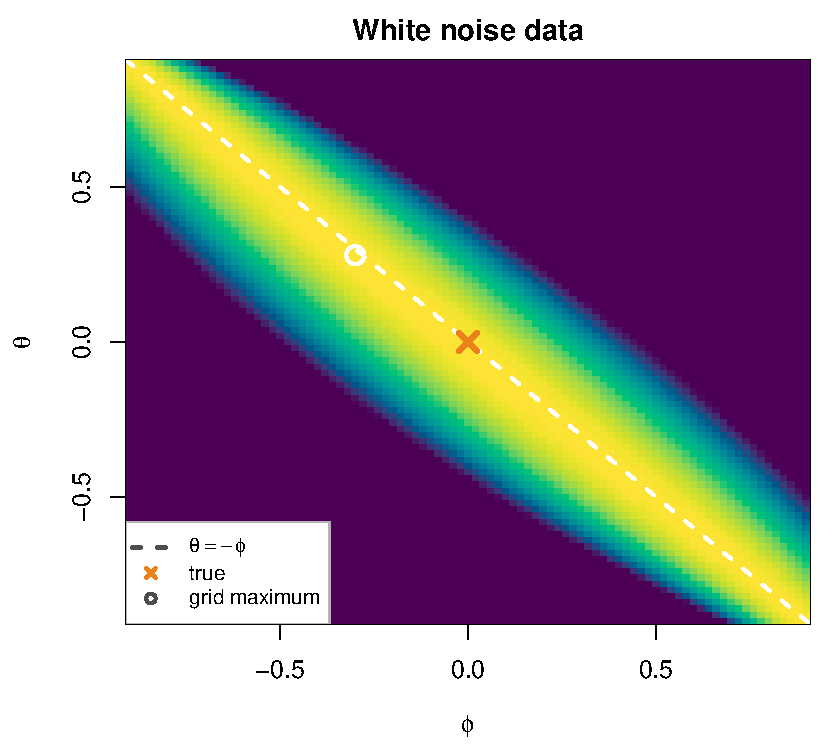
\includegraphics[width=0.49\linewidth]{figures/p3_loglik_wn.pdf}
	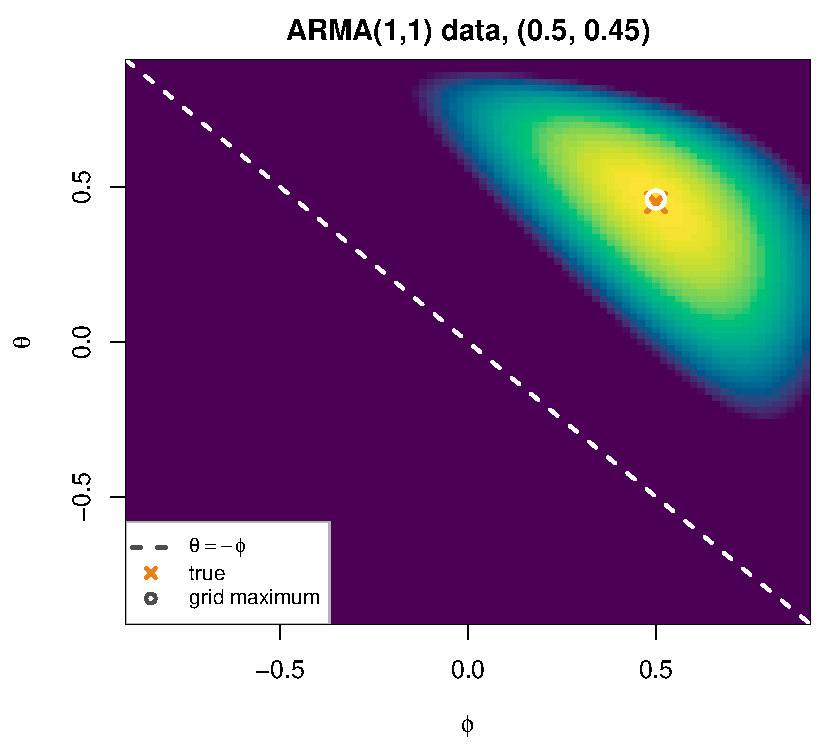
\includegraphics[width=0.49\linewidth]{figures/p3_loglik_arma.pdf}
	\caption{ARMA(1,1) log-likelihood on the grid, $T=500$, $\sigma^2=1$. Dashed: the line $\theta=-\phi$.}
	\label{fig:p3}
\end{figure}

\emph{White noise data.} The log-likelihood is a long ridge along $\theta=-\phi$. On the line it takes exactly the same value, $-721.2388942$, at $(\phi,\theta)=(-0.8,0.8)$, $(-0.4,0.4)$, $(0,0)$, $(0.4,-0.4)$ and $(0.8,-0.8)$, identical to all ten decimals. The grid maximum, $-721.06$ at $(-0.30,0.28)$, is only $0.17$ above the line: where the maximum lands along the ridge is decided by sampling noise.

\emph{Why exactly, for finite $T$.} On the line, the recursion is $\varepsilon_t=y_t-\phi y_{t-1}+\phi\varepsilon_{t-1}$. It starts at $\varepsilon_1=y_1$, because $y_0=\varepsilon_0=0$. If $\varepsilon_{t-1}=y_{t-1}$, then $\varepsilon_t=y_t-\phi y_{t-1}+\phi y_{t-1}=y_t$. So, by induction, $\varepsilon_t(\phi,-\phi)=y_t$ for every $t$ and every $\phi$, for any data. The log-likelihood on the line is that of white noise, exactly. This is an algebraic identity, not an asymptotic result.

\emph{ARMA(1,1) data with $(0.5,0.45)$.} The likelihood now has a single, well-defined peak, at $(0.50,0.46)$ on the grid, close to the truth. The line $\theta=-\phi$ is still exactly flat (the identity holds for any data), but now it is a valley: its value, $-972.4$, is $282$ log-likelihood points below the maximum, because white noise fits autocorrelated data badly. Away from cancellation, $\phi$ and $\theta$ are well identified, as c) predicts.

\lstinputlisting[caption={Problem 3 (\texttt{code/p3\_arma11\_likelihood.R})}]{code/p3_arma11_likelihood.R}

%=====================================================================
\problem

\itm{a}
At the true parameters, $\varepsilon_t$ is independent of $x_t=(1,y_{t-1})'$, with $\E[\varepsilon_t]=0$, $\E[\varepsilon_t^2]=\sigma^2$ and $\E[\varepsilon_t^4]=\kappa\sigma^4$.

\emph{Minus the expected Hessian.} The off-diagonal block is $\E[x_t\varepsilon_t]/\sigma^4=0$, and
\[
-\mathcal H_0=\begin{pmatrix}\E[x_tx_t']/\sigma^2&0\\0&-\frac1{2\sigma^4}+\frac{\E[\varepsilon_t^2]}{\sigma^6}\end{pmatrix}
=\begin{pmatrix}\E[x_tx_t']/\sigma^2&0\\0&\frac1{2\sigma^4}\end{pmatrix}.
\]
\emph{Outer product of the score.} By independence, $\E[x_tx_t'\varepsilon_t^2]/\sigma^4=\E[x_tx_t']/\sigma^2$, the same top-left block. The bottom-right entry is
\[
\E\left[\left(\frac{\varepsilon_t^2}{2\sigma^4}-\frac1{2\sigma^2}\right)^2\right]=\frac{1}{4\sigma^4}\E\left[\left(\frac{\varepsilon_t^2}{\sigma^2}-1\right)^2\right]=\frac{\kappa-2+1}{4\sigma^4}=\frac{\kappa-1}{4\sigma^4}.
\]
(The off-diagonal block of $\mathcal J_0$ is $\E[x_t]\E[\varepsilon_t^3]/(2\sigma^6)$, which is zero for symmetric shocks such as the $t$ below.) The two bottom-right entries are equal when $\frac{\kappa-1}4=\frac12$, that is, $\kappa=3$: when the shocks have the kurtosis of a normal. The information matrix equality for the mean parameters needs nothing beyond i.i.d.\ shocks; for the variance it needs the fourth moment to be right.

\itm{b}
At $\hat{\symbf\Theta}$, the OLS normal equations give $\sum_tx_t\hat\varepsilon_t=0$ and $\hat\sigma^2$ is the mean of $\hat\varepsilon_t^2$, so $\mathcal H$ is block diagonal with bottom-right entry $-1/(2\hat\sigma^4)$. The function \texttt{qmle\_ar1} below returns the three sets of standard errors. Coverage of the nominal 95\% intervals over $M=2000$ samples:

\begin{table}[H]
	\centering
	\begin{tabular}{llcccc}
		\toprule
		Shocks & $T$ & Parameter & Hessian & OPG & Sandwich \\
		\midrule
		\tablerows{tables/p4_coverage.tex}
		\bottomrule
	\end{tabular}
\end{table}

\itm{c}
With normal shocks, all intervals cover about 95\%. With $t_7$ shocks, the intervals for $c$ and $\phi$ are still fine, whatever the standard error, but the Hessian and OPG intervals for $\sigma^2$ fail: about $84\%$ and $73$--$76\%$ coverage. Only the sandwich works.

Item a) explains why. The $(c,\phi)$ block of $-\mathcal H_0$ and $\mathcal J_0$ is the same for any shock distribution, and the matrices are block diagonal, so all three variance estimators agree for $(c,\phi)$ and are all consistent. For $\sigma^2$, the correct (sandwich) asymptotic variance is
\[
\left(2\sigma^4\right)^2\cdot\frac{\kappa-1}{4\sigma^4}=(\kappa-1)\,\sigma^4,
\]
while the Hessian gives $2\sigma^4$ and the OPG gives $4\sigma^4/(\kappa-1)$. With $\kappa=5$: the truth is $4\sigma^4$, the Hessian is too small by a factor $2$ (standard error by $\sqrt2$), and the OPG by a factor $4$ (standard error by $2$). The limiting coverages are $2\Phi(1.96/\sqrt2)-1=83.4\%$ and $2\Phi(1.96/2)-1=67.3\%$. The simulated numbers are close: the Hessian is right on target, and the OPG and sandwich, which both use the fourth power of the residuals, converge slowly because $t_7$ shocks have very heavy tails (their eighth moment is infinite, so the sample kurtosis is noisy and usually too small). Intuitively, the variance of $\hat\sigma^2$ depends on how variable $\varepsilon_t^2$ is, which is a fourth-moment property; only the sandwich lets the data speak about it.

\lstinputlisting[caption={Problem 4 (\texttt{code/p4\_qmle\_ar1.R})}]{code/p4_qmle_ar1.R}

%=====================================================================
\problem

\itm{a}
Figure~\ref{fig:p5ipca} shows the series.

\begin{figure}[H]
	\centering
	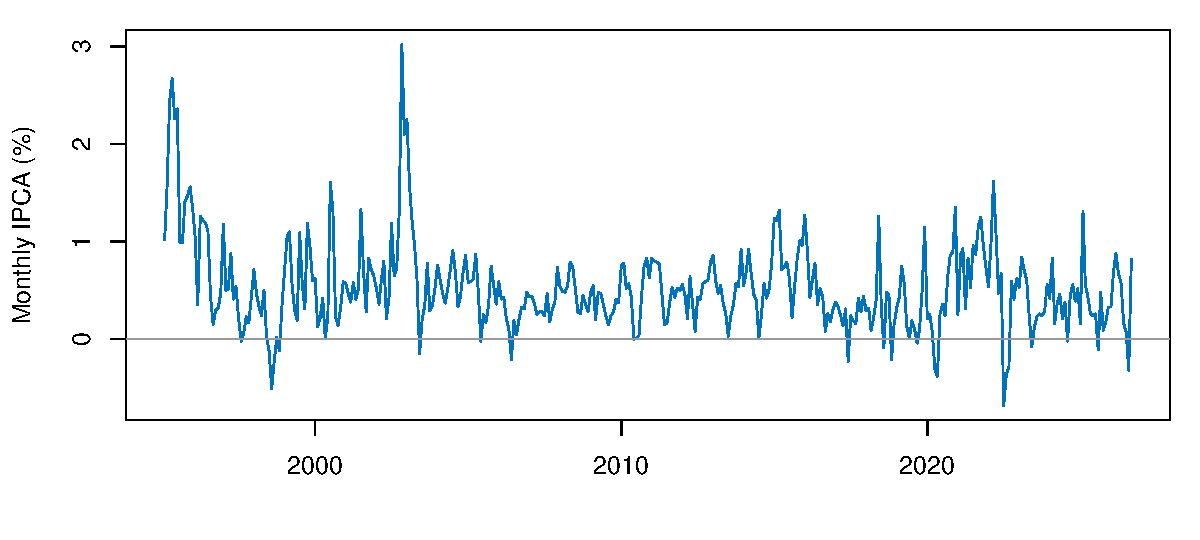
\includegraphics[width=0.9\linewidth]{figures/p5_ipca.pdf}
	\caption{Monthly IPCA (\%), February 1995 to September 2026.}
	\label{fig:p5ipca}
\end{figure}

\itm{b}
The function \texttt{loglik} in the code backs out the shocks recursively, as in Lecture 6, and returns
\[
\mathcal L(\symbf\Theta\mid\symbf y)=-\frac{n}{2}\log(2\pi\sigma^2)-\sum_{t=3}^{T}\frac{\varepsilon_t^2}{2\sigma^2},\qquad n=T-2 .
\]
All models condition on the first two observations and set the presample shocks to zero, so that every model is fit to the same $n=378$ observations and the information criteria are comparable (Lecture 6).

\itm{c}
We maximize the likelihood with $\sigma^2$ concentrated out ($\hat\sigma^2$ is the mean squared residual), from several starting points (OLS for the AR part; $0$ and $\pm0.3$ for the MA part), imposing stationarity and invertibility. The standard errors come from the inverse of minus the Hessian of $\mathcal L$, and the 95\% intervals are estimate $\pm1.96\,$se. As checks, all starting points reach the same maximum, and \texttt{stats::arima} (conditional sum of squares, same sample) gives the same estimates up to about $10^{-3}$. AIC and BIC use $k=p+q+2$ and $n=378$.

\begin{table}[H]
	\centering
	\small
	\begin{tabular}{lccccccrr}
		\toprule
		Model & $c$ & $\phi_1$ & $\phi_2$ & $\theta_1$ & $\theta_2$ & $\sigma^2$ & AIC & BIC \\
		\midrule
		\tablerows{tables/p5_models.tex}
		\bottomrule
	\end{tabular}
	\caption{Conditional ML estimates, 95\% intervals below each estimate.}
	\label{tab:p5}
\end{table}

\itm{d}
Both criteria choose the \textbf{ARMA(2,1)}, by a wide margin: its AIC is $18.7$ below the AR(1)'s and its BIC $10.8$ below. The criteria agree. But this model deserves a closer look, in the spirit of Problem 3:
\begin{itemize}
	\item Its AR polynomial has roots $1/0.875$ and $1/0.598$, and its MA root is $1/0.879$: an AR and an MA root \emph{almost cancel}. Apart from them, it is an AR(1) with coefficient $0.6$: its MA($\infty$) weights are $0.59$, $0.35$, $0.21$, \dots, almost exactly $0.6^j$. Its implied autocorrelations are not closer to the data than the AR(1)'s; if anything, they decay a bit too fast (Figure~\ref{fig:p5acfmodels}). So its better fit does not come from better dynamics.
	\item Its likelihood gain over the AR(1), $11.3$ points, comes almost entirely from 1995--96 ($9.0$ points). With exactly cancelling roots, $(1-\rho L)(1-aL)y_t=c+(1-\rho L)\varepsilon_t$, the recursion started at $\varepsilon_2=0$ gives $\varepsilon_t=x_t-\rho^{\,t-2}x_2$, where $x_t$ is the AR(1) residual. The conditional likelihood then fits a geometrically decaying ``initial condition'' for free, and in 1995 inflation was far above its mean, falling fast after the Real Plan. The near-cancelling pair is soaking up that disinflation.
	\item Starting the sample in January 2000, both criteria choose the AR(1), and the ARMA(2,1) gains only $0.05$ log-likelihood points over it. On the full sample with the exact likelihood, which does not set presample shocks to zero, the ARMA(2,1) does not improve on the AR(1) at all (log-likelihoods $-123.91$ and $-123.92$).
	\item The ARMA(2,2), second by both criteria, has the same nearly cancelling pair (inverse roots $0.871$ and $0.878$).
\end{itemize}
\begin{figure}[H]
	\centering
	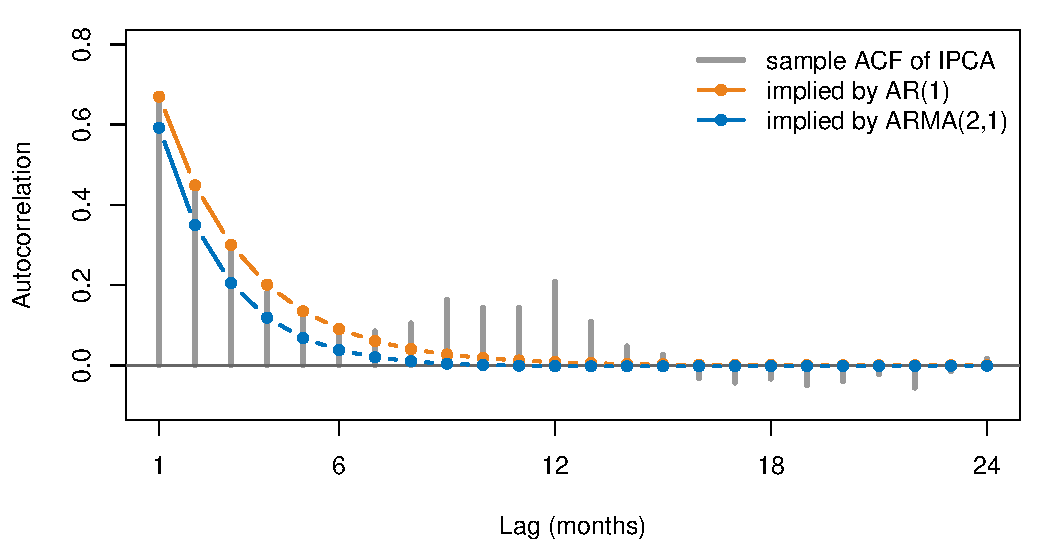
\includegraphics[width=0.7\linewidth]{figures/p5_acf_models.pdf}
	\caption{Sample autocorrelations of IPCA and those implied by the estimated AR(1) and ARMA(2,1).}
	\label{fig:p5acfmodels}
\end{figure}
So we pick the \textbf{AR(1)}: $\hat y_t=0.173+0.670\,y_{t-1}$, $\hat\sigma^2=0.111$, with an implied mean of $0.523\%$ per month. Among the models without redundant roots, it has the lowest BIC, and its AIC is within $0.4$ of the lowest (the ARMA(1,2)'s, whose MA coefficients are imprecise: $\theta_2$ is not significant and $\theta_1$ only barely). Its dynamics are also what the ARMA(2,1) uses away from the start of the sample. (The fitted values and forecasts below would barely change with the ARMA(2,1), since the transient has long died out by the end of the sample.)

\itm{e}
Figure~\ref{fig:p5fit} plots the fitted values, $\hat y_t=y_t-\hat\varepsilon_t$, and the residuals of the AR(1).
\begin{figure}[H]
	\centering
	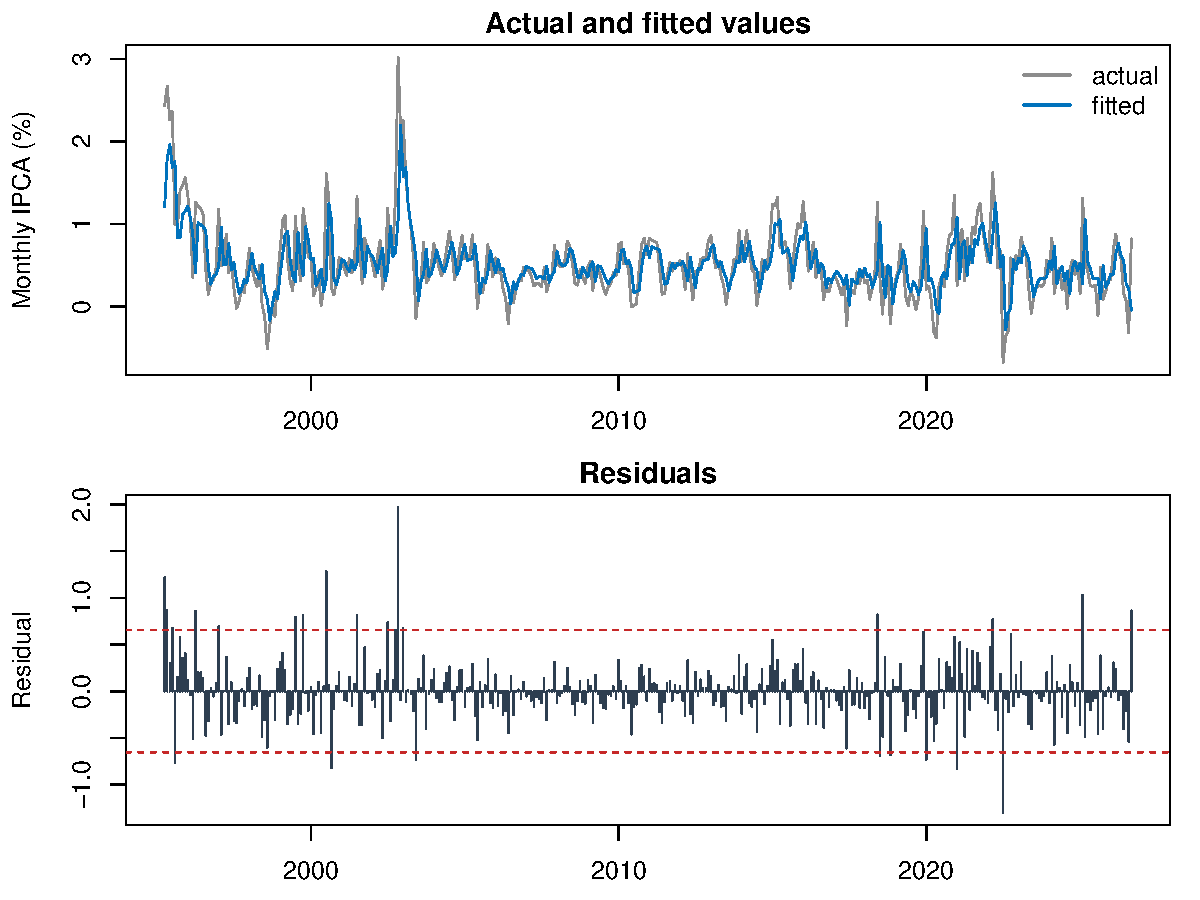
\includegraphics[width=0.9\linewidth]{figures/p5_fit.pdf}
	\caption{AR(1): fitted values and residuals. The dashed lines are $\pm1.96\,\hat\sigma$.}
	\label{fig:p5fit}
\end{figure}
The fitted values follow the series with a one-month delay: they are a shrunk version of last month's inflation, $0.173+0.67\,y_{t-1}$. The model gets the persistence right but cannot anticipate turning points or spikes, such as the jump at the end of 2002 or the deflation of mid-2022. The residuals have no visible trend, but they are not i.i.d.\ normal:
\begin{itemize}
	\item they are heteroskedastic: their standard deviation is $0.41$ in 1995--99, $0.33$ in 2000--09, $0.25$ in 2010--19 and $0.38$ in 2020--26;
	\item they have fat tails and positive skewness (kurtosis $7.3$, skewness $0.9$), with outliers such as November 2002 ($+2.0$) and July 2022 ($-1.3$, after the cuts in fuel and electricity taxes).
\end{itemize}
So the Gaussian likelihood is really a quasi-likelihood. By Problem 4, the intervals for $c$ and $\phi$ in Table~\ref{tab:p5} are still reasonable, but the one for $\sigma^2$ is too narrow; a sandwich would fix it.

\itm{f}
Figure~\ref{fig:p5acf} shows the residual autocorrelations up to lag 24.
\begin{figure}[H]
	\centering
	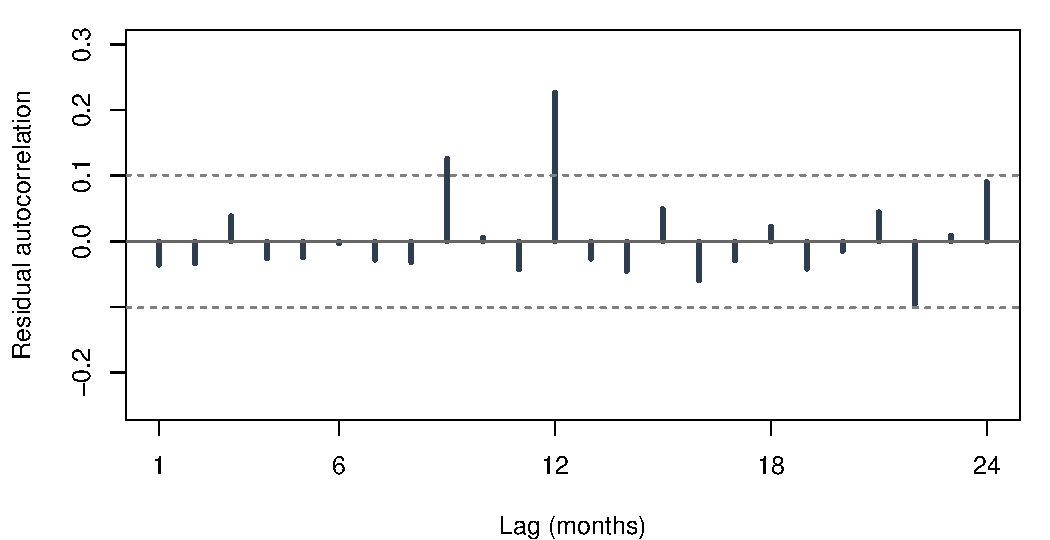
\includegraphics[width=0.7\linewidth]{figures/p5_resid_acf.pdf}
	\caption{Autocorrelation of the AR(1) residuals; dashed lines: $\pm1.96/\sqrt n$.}
	\label{fig:p5acf}
\end{figure}
There is no autocorrelation left at short lags: the first eight residual autocorrelations are all below $0.04$ in absolute value. The AR(1) captures the short-run dynamics. But there are spikes at lag 9 ($0.13$) and, especially, lag 12 ($0.23$), outside the bands, and the Ljung--Box test with 24 lags rejects white noise ($p=0.009$). This is the seasonality from Problem Set II, Problem 6. An ARMA with $p,q\le2$ cannot capture it: its autocorrelations decay geometrically after lag $q\le2$, so it cannot produce a spike at lag 12 next to near-zero autocorrelations at lags 3--11. A seasonal term (an AR coefficient at lag 12) or month dummies would be the next step.

\itm{g}
Figure~\ref{fig:p5path} shows one simulated path. Each simulated value is $y_{T+h}=\hat c+\hat\phi\,y_{T+h-1}+\varepsilon_{T+h}$, with $\varepsilon_{T+h}\sim N(0,\hat\sigma^2)$, starting from the last observation (September 2026: $0.82\%$). A single path looks like the data: persistent, noisy, and with no tendency to stay near the forecast mean.
\begin{figure}[H]
	\centering
	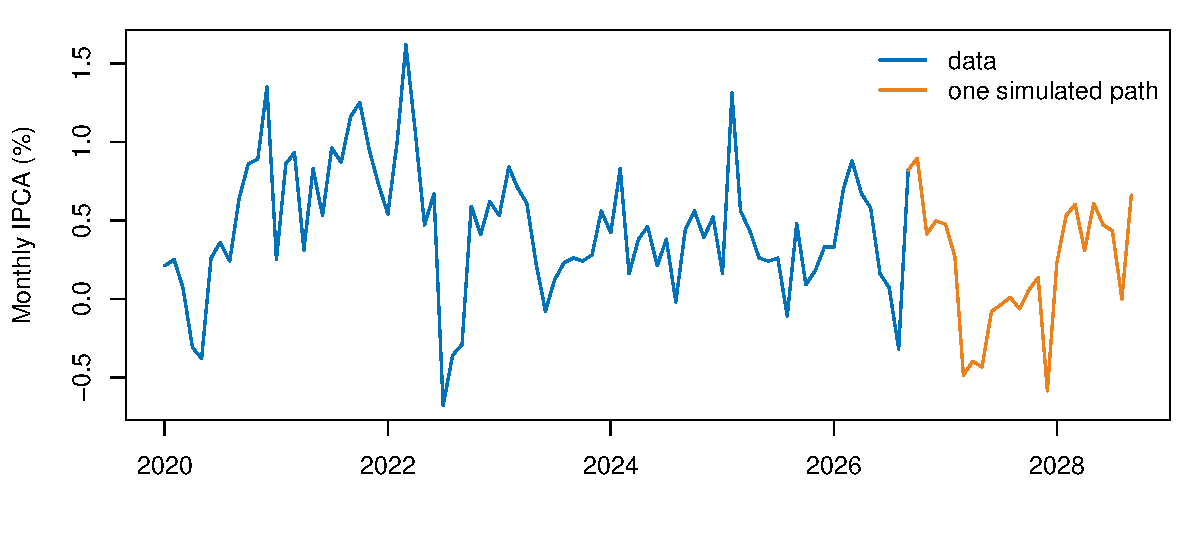
\includegraphics[width=0.85\linewidth]{figures/p5_one_path.pdf}
	\caption{The series since 2020 and one simulated 24-month path.}
	\label{fig:p5path}
\end{figure}

\itm{h}
Figure~\ref{fig:p5fan} summarizes 1000 simulated paths.
\begin{figure}[H]
	\centering
	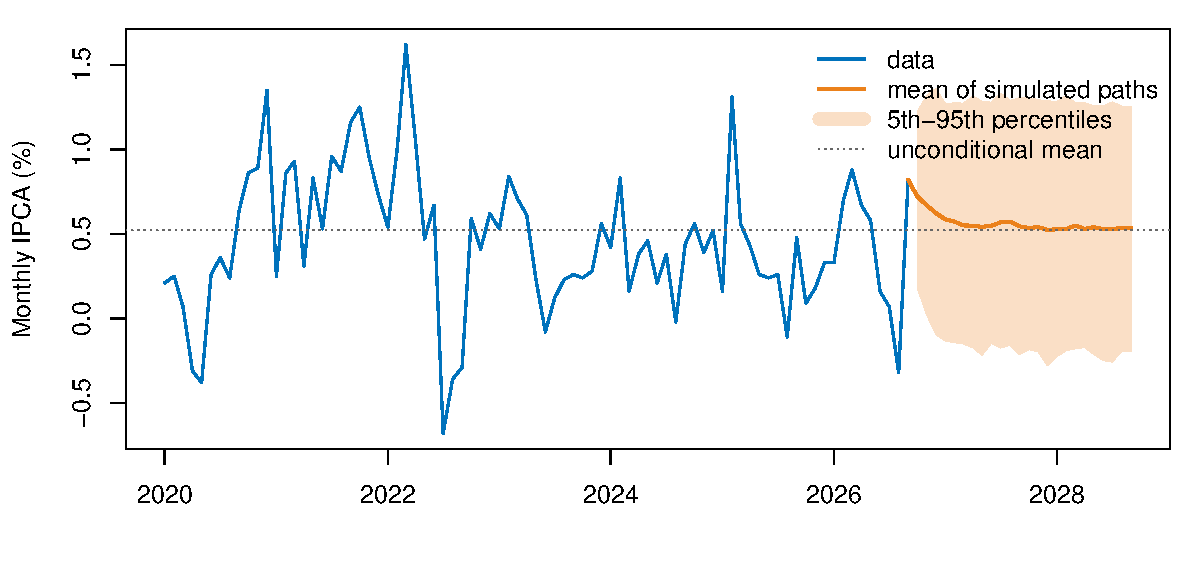
\includegraphics[width=0.85\linewidth]{figures/p5_fan.pdf}
	\caption{Mean of 1000 simulated paths and their 5th and 95th percentiles.}
	\label{fig:p5fan}
\end{figure}
The mean of the simulated paths starts at $0.72\%$ one month ahead and decays toward the model's mean, $0.52\%$, at rate $\hat\phi^h$. It is within $0.02$ of the mean after a year. The 5th--95th percentile band is $[0.18,1.23]$ one month ahead and widens to about $[-0.2,1.3]$, the unconditional 90\% range of the model, within six months or so. This is Problem 1 f) in action: as $h$ grows, the conditional mean and variance converge to the unconditional ones, and the forecast stops using what we know today.

\itm{i}
The idea is the same as in the bootstrap: we do not know the distribution of future inflation, so we estimate the data-generating process and simulate from the estimate, then read uncertainty off the simulated draws. But there are two differences:
\begin{itemize}
	\item This is a \emph{parametric} bootstrap: the shocks come from the fitted $N(0,\hat\sigma^2)$, not from the empirical distribution. The nonparametric analogue would resample the estimated residuals with replacement, which would carry over the fat tails and skewness of e) into the bands.
	\item It treats $\hat{\symbf\Theta}$ as the truth, so it ignores estimation uncertainty and the bands are somewhat too narrow. To include it, re-estimate the model on each simulated sample (or draw $\symbf\Theta$ from its estimated asymptotic distribution) before simulating forward.
\end{itemize}
Note also that the target is different: these bands are prediction intervals for a future random value, not confidence intervals for a fixed parameter.

\lstinputlisting[caption={Problem 5 (\texttt{code/p5\_ipca\_arma.R})}]{code/p5_ipca_arma.R}

\end{document}
